\section{Results} \label{sec:results}
This project came bundled with a lot of known unknowns and, as I would soon discover, even more unknown unknowns. Since a major part of this project was about learning the ropes of MLIR, this section will present results related to the implementation and the development process.

\subsection{Building}
The first step was to actually build the baseline project. A warning will show up when attempting to build the jlm eval suite, telling the user that at least 16 GB of memory is needed to complete the build. I first tried to build on my desktop PC, which has 16 GB of memory, but it froze almost immediately. I decided to leave it on overnight just to see if it might work, but after approximately 36 hours of building and no apparent progress, I pulled the plug. After getting access to a machine with 32 GB of memory and 6 cores, things worked more smoothly, but build times for pristine builds were still in the order of 4 hours. Incremental builds were more manageable at around 5 minutes. While no comprehensive profiling was done of the build process, it seemed like rebuilding MLIR took up most of the time.

\subsection{Project structure} \label{sec:results:project-structure}
The next step was getting to know MLIR. That meant figuring out what needed to be done to implement a new dialect and how to best implement RVSDG using the framework provided by MLIR. There are a couple of different ways a dialect can be defined. They can either be defined directly by implementing a set of C++ templates, or declaratively using TableGen \cite{mlir_tablegen_ods}. Using TableGen has the benefit of automatically generating a lot of the necessary boilerplate code needed to cleanly interface with Ops once they have been properly specified. It is also meant to provide a single source of truth for all facts surrounding Ops. TableGen does however come with a quite high buy-in cost for first-time users, as it is an entire new programming language that needs to be learned. I decided to go the TableGen route, since the MLIR documentation was quite adamant about TableGen being the recommended way to define pretty much anything.

As for the structure of the project itself, there are two main ways to do it: standalone or in-tree. Standalone dialects are usually hosted in their own repository and import an external copy of MLIR. Structuring a project in this way keeps all files related to the specific dialect separated from the in-tree dialects. It also doesn't require the developer to work on a custom version or fork of LLVM just to make their one-time use dialect. The main drawback of standalone dialects is that they are not included into MLIR's default tooling, which means that some tools will have to be explicitly extended by the dialect author. There is also some extra investment into setting up build infrastructure for the dialect and the application that will use it.

The other way to structure a dialect is to make it in-tree. This means that the dialect lives in the MLIR source tree together with the default dialects. An in-tree setup has a few advantages over a standalone setup. The first, and most obvious one, is that it is much easier to integrate into upstream MLIR. There is also a larger amount of easily accessible examples on how to set up an in-tree dialect. Setting up dialect building is also easier, as CMakeLists can be more or less copied from the default dialects. The cons of structuring a dialect like this are substantial, however. Source files get spread out across many different directories, causing development to take longer as the dialect author needs to navigate back and forth into somewhat deeply nested directory trees. The build system for the dialect also ends up being very fractured. Perhaps the biggest con though is that any change to the dialect triggers a rebuild of all of MLIR. Not a clean build, mind you, but it still re-tests and re-links many libraries and tools. Build errors also cause long cryptic error messages that can be really hard to track down since they usually appear in auto-generated files. Another problem is that if a user wished to use two in-tree non-default dialects, they would either need to combine the two modified MLIR repositories themselves, or build two separate versions of MLIR and link in both. Neither of those are good options.

I decided to go for an in-tree structure for the RVSDG dialect due to the ease of finding examples and because the main MLIR dialect implementation tutorial used this structure \cite{noauthor_creating_nodate}.

\subsection{Chosen representations} \label{sec:chosen-representations}
A major part of this project was to figure out how RVSDG concepts can be represented in MLIR. The first concept I decided to tackle was nodes. RVSDG nodes map quite nicely to MLIR Ops. They both take inputs, produce outputs, and can contain structural regions. Edges between nodes can then be represented by passing MLIR SSA-values that are the output of one Op to the input of another Op. Using this abstraction has the added benefit of enabling Ops from other dialects to act as simple nodes, which saves development effort for implementing arithmetic operations, constant materialization, string operations etc. By itself, it unfortunately does not enable the representation of state edges. How this could be done will be discussed in section \ref{sec:future-work:copleting-representations}.

The above representation should be able to handle inputs and outputs quite nicely, but arguments and results still need to be represented. Currently, arguments are handled by allowing only SSA-values passed as inputs to the structural node to be accessed in the contained region. This method works fine for \hyperref[lbl:gamma-node]{gamma-nodes}, but for most other nodes this way of handling arguments will not work as there is not a one-to-one mapping between inputs and arguments. Results are handled using an MLIR terminator Op, with the result values being passed as arguments. A better way to handle arguments and results will be discussed in section \ref{sec:future-work:copleting-representations}.

MLIR regions themselves come in several different flavours, the main two being SSACFG and graph regions \cite{mlir_lang_ref}. I chose to use SSACFG regions to model RVSDG regions, which might seem like an odd choice. After all, graph regions specifically provide semantics that are geared towards implementing data dependence graphs and similar constructs. The reason I decided against graph regions is that their primary feature is to allow for cyclic data dependencies. This is not a desirable property in RVSDG as it should always be acyclic, so we get more semantics for free by using SSACFG regions. Graph regions also don't allow for block arguments, which might be required for future work as discussed in \autoref{sec:future-work:copleting-representations}.

\subsection{Printing and parsing}
A lot of development time was spent hooking into the printing and parsing infrastructure for MLIR's textual representation. This was done to be able to quickly create nodes and see if they behaved as expected under different operations. Being able to print them out also made it a lot easier to see what was actually going on while developing. MLIR does provide a default textual representation for all Ops, which I could have used. Instead, I chose to use a custom assembly format to make it easier to read and write the MLIR assembly. 

There are two ways to create a custom assembly format for an Op. The first one is by using MLIRs declarative assembly format. This mechanism allows the Op author to define the format of their Op by writing a string representation of the format of the Op in the Ops TableGen definition. This string is written using a combination of literals and directives. Literals are literal pieces of text that should be part of the format \cite{mlir_declarative_assembly_format}. Directives are functions which can optionally take arguments. The built-in directives primarily handle basic printing and parsing of necessary values such as operands, results, types, attributes etc. It is also possible to define custom directives which allows for more specialized printing of certain parts of the Op, while largely retaining the ease of readability and modifiability that the declarative format offers.

If custom directives are not enough, MLIR also offers Op authors the option to create their own printers and parsers from scratch. These are implemented as class methods on the Op's C++ class. MLIR can automatically generate definitions for these methods if specified to in the Op's TableGen definition. MLIR offers some useful helper functions for printing and parsing common patterns such as operands, types, and attributes, which the Op author may use in their own printer/parser. Due to the nature of these methods as fully customizable, there aren't really any solid guidelines for how to create them, but parsers must eventually call the Op's build method to create the Op instance.

I decided to use the declarative format since it required less boilerplate. I didn't quite like the way it printed operands and their types. Using the pure declarative format, variadic operands had to be printed as a list of SSA-values with a separate list of types. This separation of operands and types made the assembly harder to read and, in my opinion, less aesthetically pleasing. To get around this, I implemented a custom directive that prints the list of operands in the format "(operand0: type0, operand1: type1, ...)". This was significantly less work than implementing an entire custom printer/parser-pair for the entire Op, and still made the assembly format prettier and more semantically coherent.

\subsection{Implemented features}
At the current state of development, a few things have been accomplished. The first, and arguably most important milestone is that the RVSDG dialect itself is getting built and registered in MLIR. Doing this both required hooking into MLIRs CMakeLists and modifying some core MLIR tools to let use the RVSDG dialect. Doing this was necessary to test my implementations in isolation.

Although the dialect itself is registered, it is not even close to complete. As of writing this, the only node that has been properly implemented is the \hyperref[lbl:gamma-node]{gamma-node}. It uses the representations mentioned above and is fully compatible with other MLIR assembly. A few unit tests have also been written, including a round-trip test which helps ensure that the node is not accidentally broken during development. Some initial work has also been done on the lambda-node, but time ran out before it could be completed.

\begin{figure}[H]
    \centering
    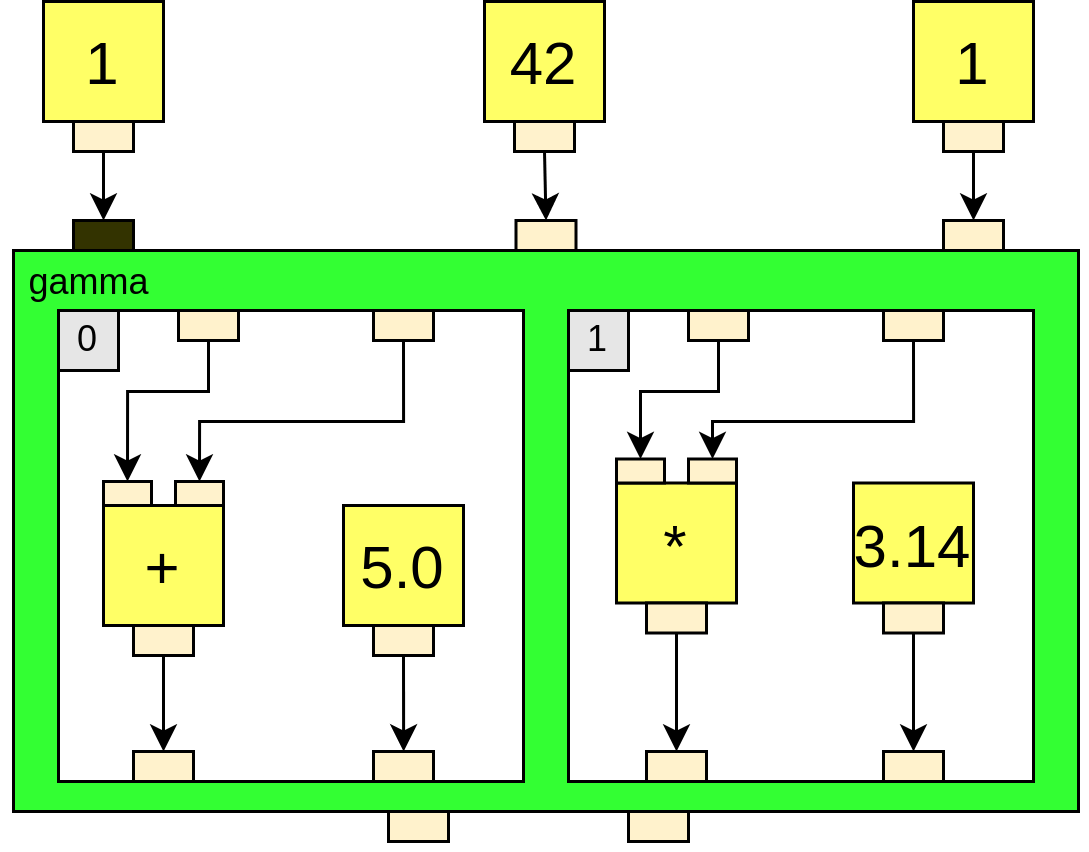
\includegraphics[width=\textwidth/3]{Images/example_mlir_assembly_cropped.png}
    \begin{minted}[fontsize=\footnotesize]{text}
%predicate = arith.constant 1: index
%in_0 = arith.constant 42: i32
%in_1 = arith.constant 1: i32

%out0, %out1 = rvsdg.gammaNode (%predicate) 
(%in_0: i32, %in_1: i32): [
    {
        %res_0 = arith.addi %in_0, %in_1 : i32
        %res_1 = arith.constant 5.0: f64
        rvsdg.gammaOutput(%res_0: i32, %res_1: f64)
    },
    {
        %res_0 = arith.muli %in_0, %in_1 : i32
        %res_1 = arith.constant 3.141: f64
        rvsdg.gammaOutput(%res_0: i32, %res_1: f64)
    }
] -> i32, f64
    \end{minted}
    \caption{Representation of a gamma-node and some simple nodes as MLIR assembly.}
    \label{fig:my_label}
\end{figure}
